\documentclass[a4paper, 12pt]{article}
\usepackage[T2A,T1]{fontenc}
\usepackage[utf8]{inputenc}
\usepackage[english, russian]{babel}
\usepackage{graphicx}
\usepackage[hcentering, bindingoffset = 10mm, right = 15 mm, left = 15 mm, top=20mm, bottom = 20 mm]{geometry}
\usepackage{multirow}
\usepackage{lipsum}
\usepackage{amsmath, amstext}
\usepackage{siunitx}
\usepackage{subcaption}
\usepackage{wrapfig}
\usepackage{mathrsfs}
\usepackage{adjustbox}
\usepackage{enumerate, indentfirst, float}
\usepackage{capt-of, svg}
\usepackage{icomma}
\usepackage{xcolor}

\newenvironment{bottompar}{\par\vspace*{\fill}}{\clearpage}
 
\begin{document}
\begin{titlepage}

\newcommand{\HRule}{\rule{\linewidth}{0.5mm}} % Defines a new command for the horizontal lines, change thickness here

\center % Center everything on the page
 
%----------------------------------------------------------------------------------------
%	HEADING SECTIONS
%----------------------------------------------------------------------------------------

\textsc{\LARGE Московский Физико-Технический Институт}\\[1,5cm] % Name of your university/college
\textsc{\Large Кафедра общей физики}\\[0.5cm] % Major heading such as course name
\textsc{\large Лабораторная работа \textnumero  3.3.4}\\[0.5cm] % Minor heading such as course title

%----------------------------------------------------------------------------------------
%	TITLE SECTION
%----------------------------------------------------------------------------------------

\HRule
\\[0.4cm]
{ \huge \bfseries Эффект Холла в полупроводниках}
\\[0.2cm] % Title of your document
\HRule
\\[1.5cm]


 
%----------------------------------------------------------------------------------------
%	AUTHOR SECTION
%----------------------------------------------------------------------------------------

\begin{minipage}{0.4\textwidth}
	\begin{flushleft} \large
		\emph{Автор:}\\
		Ришат \textsc{Исхаков} \\
		513 группа
	\end{flushleft}
\end{minipage}
~
\begin{minipage}{0.4\textwidth}
	\begin{flushright} \large
		\emph{Преподаватель:} \\
		Александр Александрович \textsc{Казимиров} % Supervisor's Name
	\end{flushright}
\end{minipage}

\begin{bottompar}
	\begin{center}
		
\includegraphics[width = 80 mm]{logo.jpg}
	\end{center}
	{\large \today}

\end{bottompar}
\vfill % Fill the rest of the page with whitespace

\end{titlepage}

\section{Цель работы}
Измерение подвижности и концентрации носителей заряда в полупроводниках.

В работе используются: \textit{электромагнит с источником питания, амперметр, миллиамперметр, милливеберметр, реостат, цифровой вольтметр, источник питания, образцы легированного германия.}


\subsection*{Теоретическая часть}

\subsubsection*{Дырки}

Эффект Холла, возникающий в проводниках, происходит из-за наличия некоторого количества свободных электронов в зоне проводимости и такого же количества дырок в валентной зоне. Чтобы понять причину образования дырок, нужно рассмотреть дырочную проводимость.


Дырочную проводимость можно объяснить при помощи следующей аналогии: если представить ряд людей, сидящих в аудитории, где нет запасных стульев. Когда кто-нибудь из середины ряда хочет уйти, он      перелезает через спинку стула в пустой ряд и уходит. Здесь пустой ряд — аналог зоны проводимости, а ушедшего человека можно сравнить со свободным электроном.
Теперь представим, что ещё кто-то пришёл и хочет сесть. Из пустого ряда плохо видно, поэтому там он не садится. Вместо этого человек, сидящий возле свободного стула, пересаживается на него, вслед за ним это повторяют и все его соседи. Таким образом, пустое место как бы двигается к краю ряда. Когда это место окажется рядом с новым зрителем, он сможет сесть.
В этом процессе каждый сидящий передвинулся вдоль ряда. Если бы зрители обладали отрицательным зарядом, такое движение было бы  \textit{электрической проводимостью}. Если вдобавок стулья заряжены положительно, то ненулевым суммарным зарядом будет обладать только свободное место. Это простая модель, показывающая как работает \textit{дырочная проводимость}. Однако на самом деле, из-за свойств кристаллической решётки, дырка не локализована в определённом месте, как описано выше, а размазана по области размером во много сотен элементарных ячеек.

\subsubsection*{Эффект Холла}


\begin {figure}[H]
	\begin{center}
		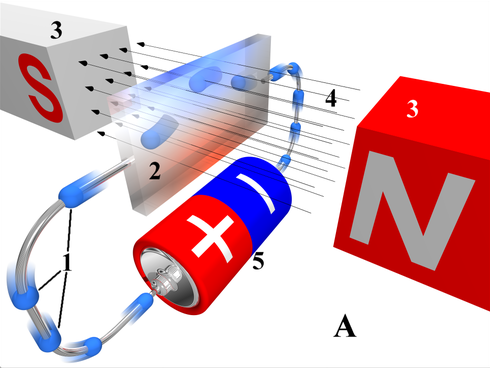
\includegraphics[width = 0.6 \textwidth]{Hall_effect}
		\caption{Пример действия эффекта Холла на свободные заряды}
	\end{center}
\end {figure}


Магнитного поле в проводнике действует на свободные электроны в зоне проводимости, поэтому между гранями наблюдается добавочная разность потенциалов, связанная с силой Лоренца. 

$$\boldsymbol{F_\text{Л}}  = -e \boldsymbol{E} - e \langle \boldsymbol{\upsilon} \rangle \times \boldsymbol{B},$$
где $e$ - абсолютная величина заряда электрона, $\boldsymbol{B}$ - индукция магнитного поля, $\boldsymbol{E}$ - напряженность электрического поля, $ \langle \upsilon \rangle$ - средняя скорость заряда.

Из этого выражения получим разность потенциалов между двумя гранями:

\begin{equation}
U = -E_zl = - | \langle \upsilon \rangle | B l
\label{eq:pot_dif}
\end{equation}

С этой возникшей разностью потенциалов и связан Эффект Холла.

Далее, если выразить ток:
$$ I = ne |\langle \upsilon \rangle |  l a$$
И совместить его с \ref{eq:pot_dif}, получим ЭДС Холла:

\begin{equation}
\mathscr{E}_x = U = - \dfrac{IB}{nea} = -R_x \cdot \dfrac{IB}{a},
\label{eq: Hall}
\end{equation}

где $R_x = \dfrac{1}{ne}$ называется \textit{постоянной Холла.}

\subsection*{Установка и параметры измерения}

\begin{wrapfigure}[15]{l}{0.7 \textwidth}
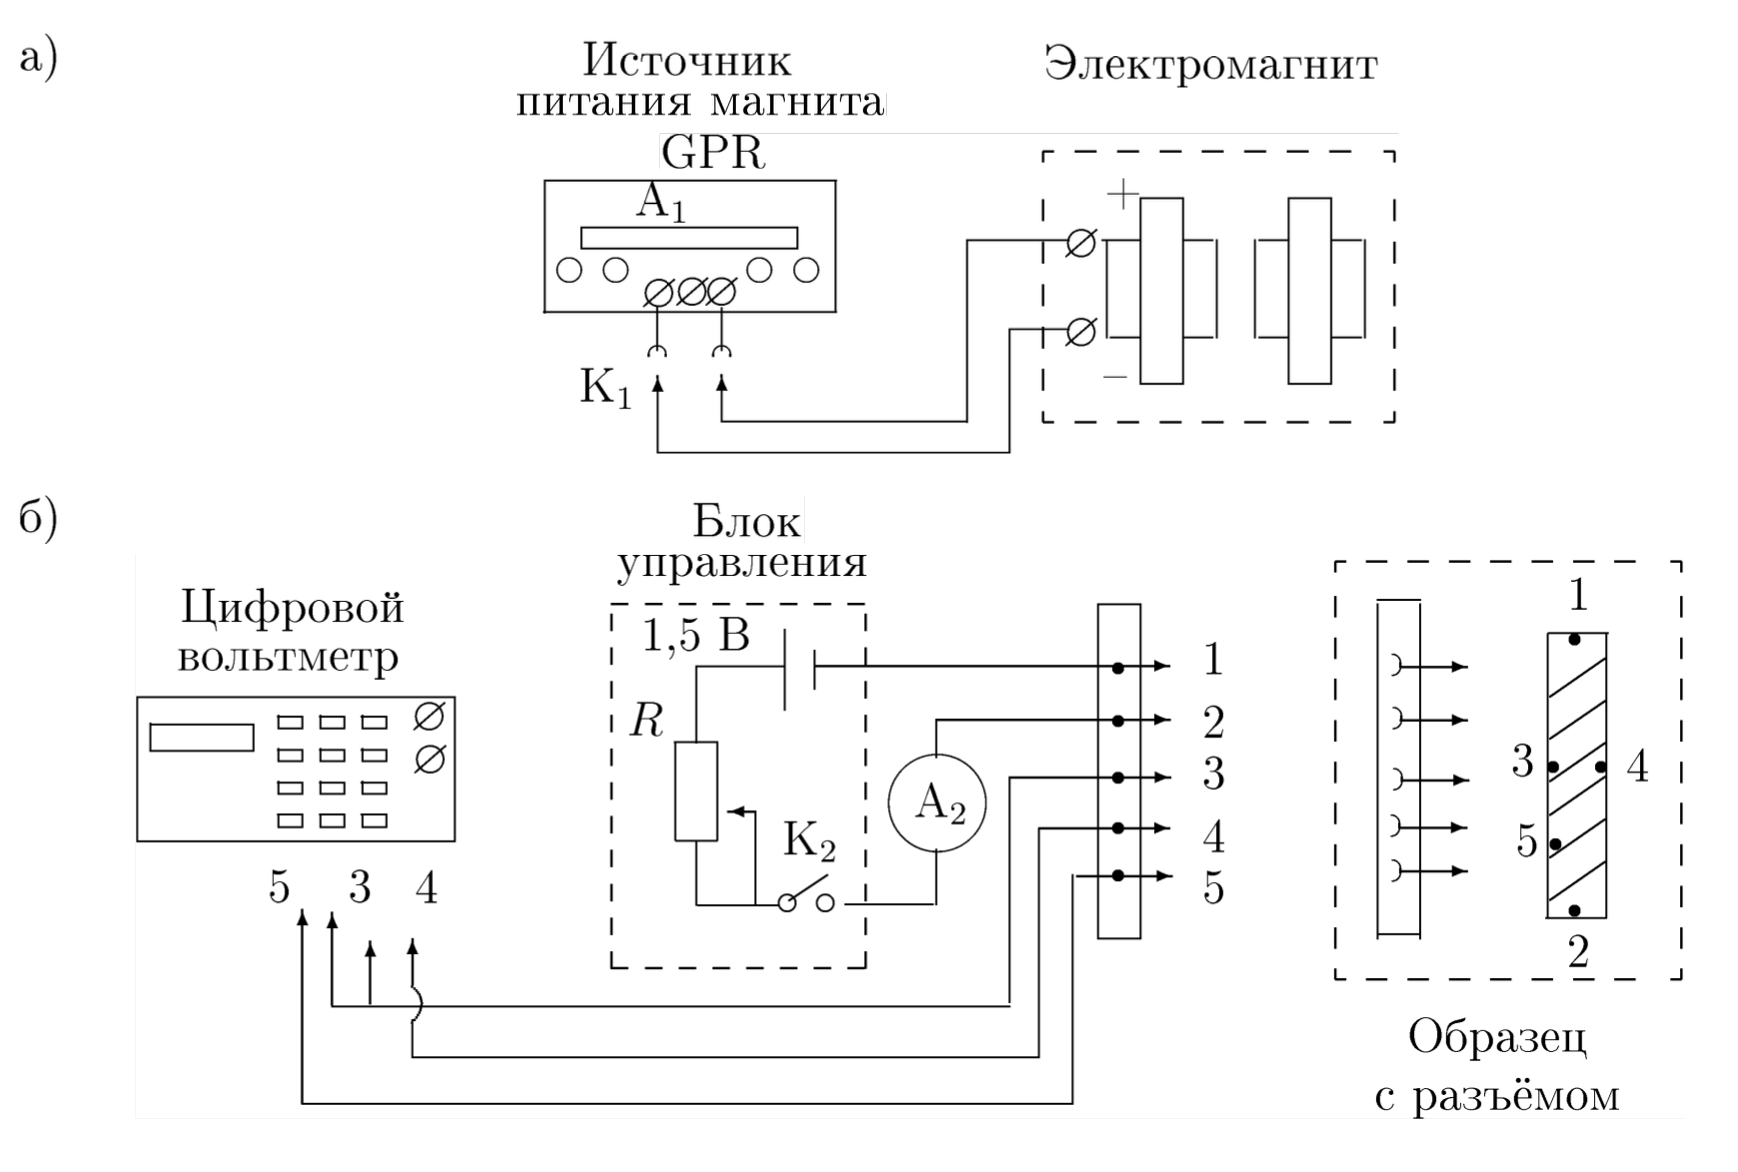
\includegraphics[width = 0.7 \textwidth]{Scheme1}
			\caption{Схема установки для измерения эффекта Холла в полупроводниках}
\end{wrapfigure} 

		$$\text{Параметры установки:}$$
$$a = 2.2 \text{ мм}$$
$$L_{35} = 3 \text{ мм}$$
$$l = 2.5 \text{ мм}$$
\vspace{5 cm}

В нашей установке вдоль длинной стороны образца будет течь ток, величина которого регулируется реостатом $R_2$. Так как он помещен в электромагнит, между точками \textit{3 и 4} будет возникать разность потенциалов $U_{34}$, которую мы будем измерять. 

Однако между точками \textit{3 и 4} будет возникать некоторое дополнительное падение напряжения $U_{0}$, так как эти точки оказываются не на одной эквипотенциали. Исключить это влияние можно с помощью изменения направления магнитного поля: в одном случае $U_{34} = U_{0} - \mathscr{E}_x $, в другом  $U_{34} = U_0 - \mathscr{E}_x $. Тогда с помощью полуразности избавимся от $U_{0}$ в наших измерениях. 

\begin{figure}[H]
	\begin{center}
		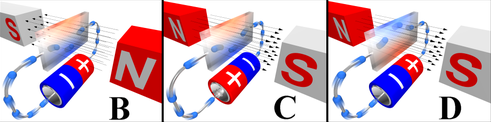
\includegraphics[width = 0.6 \textwidth]{Hall_dif}
		\caption{Эффект Холла при различных направлениях магнитного поля и тока через образец}
	\end{center}
\end{figure}

\section{Работа и измерения}

\subsection*{Калибровка установки}

\begin{table}[H]
\centering
\begin{tabular}{|c|c|c|c|c|c|c|c|c|c|}
\hline
$I, \text{ мА}$ & 0    & 0.1   & 0.4 & 0.6   & 0.8   & 1     & 1.2    & 1.4    & 1.6    \\ \hline
$B, \text{ Тл}$ & 22.4 & 115.8 & 431 & 616.5 & 791.2 & 912.4 & 1000.5 & 1061.5 & 1107.9 \\ \hline
\end{tabular}
\caption{Данные для калибровки установки}
\end{table}

	\begin {figure}[H]
		\begin{center}
			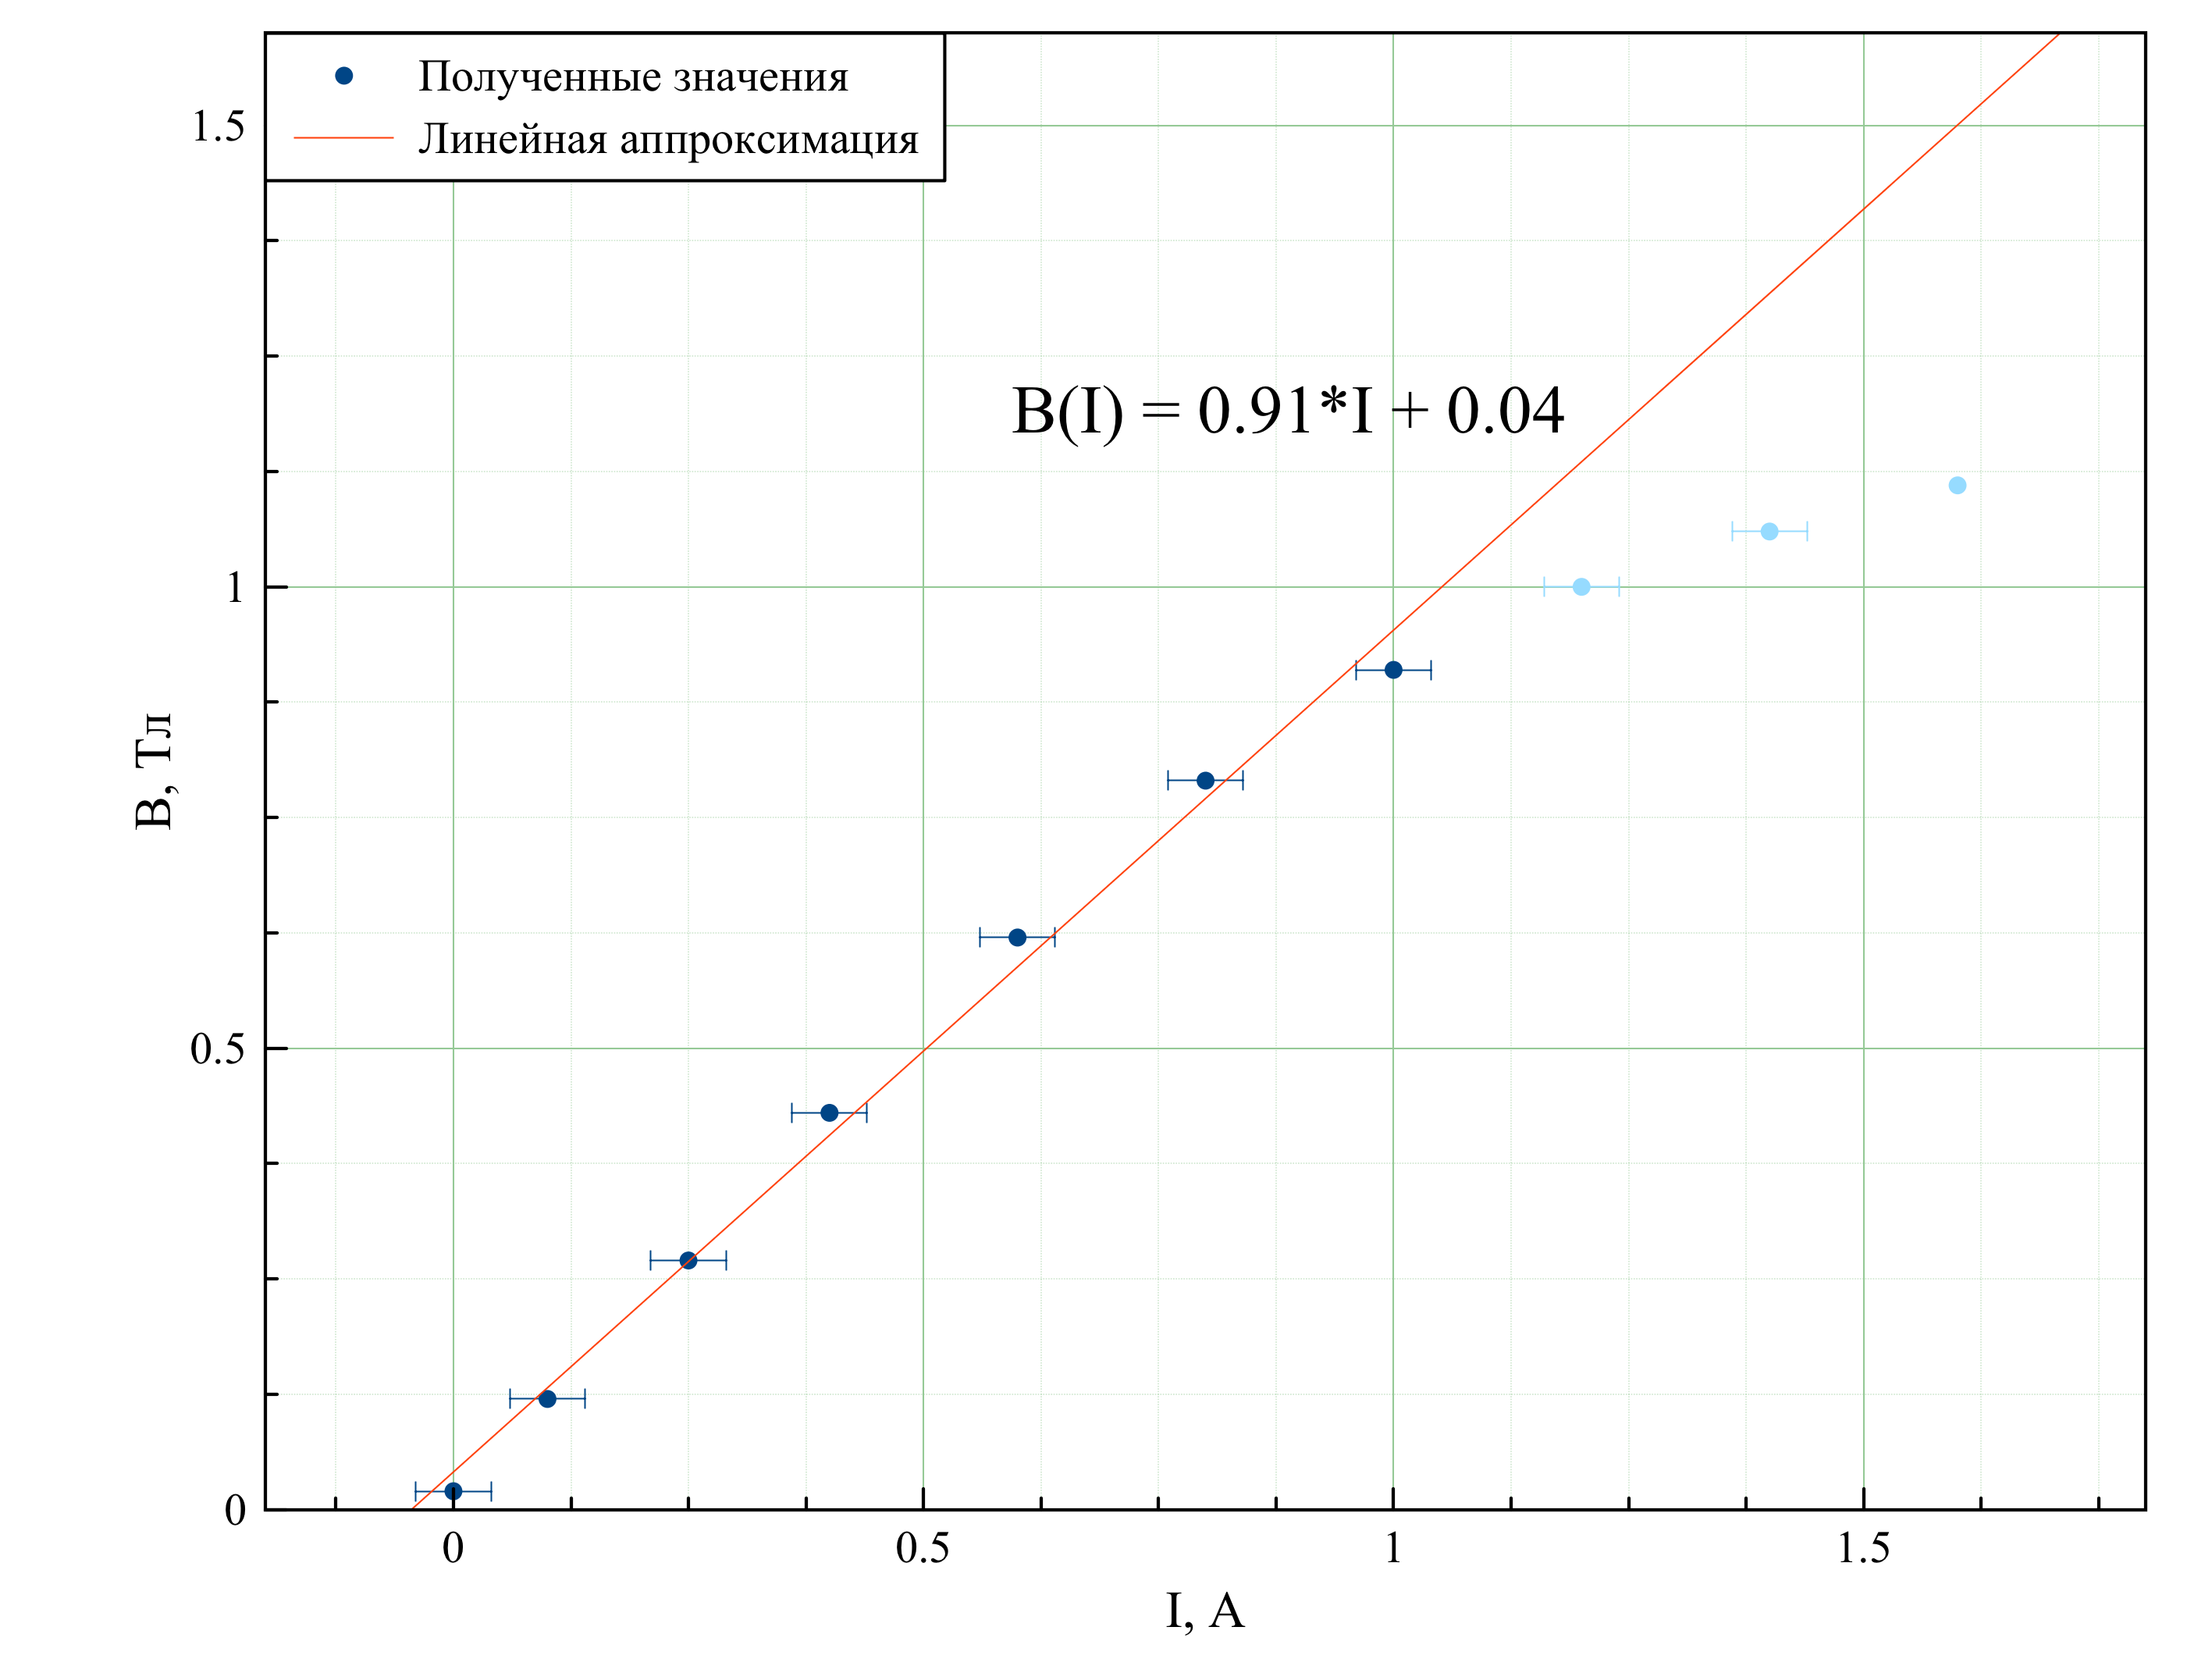
\includegraphics[width = 0.9 \textwidth]{Equation}
			\caption{Уравнение для калибровки установки}
		\end{center}
	\end {figure}

\begin{table}[H]
\centering
\resizebox{\textwidth}{!}{%
\begin{tabular}{|c|c|c|c|c|c|c|c|c|c|c|}
\hline
                                  &                                     & $I_M, \text{ А}$                                  & 0.1                           & 0.2                           & 0.3                           & 0.4                           & 0.5                           & 0.6                           & 0.8                           & 1                             \\ \cline{3-11} 
\multirow{-2}{*}{$I, \text{ мА}$} & \multirow{-2}{*}{$U_0, \text{ мВ}$} & $B, \text{ Тл}$                                   & 0.131                         & 0.222                         & 0.313                         & 0.404                         & 0.495                         & 0.586                         & 0.768                         & 0.95                          \\ \hline
{\color[HTML]{31A4FF} 0.3}        & {\color[HTML]{31A4FF} -0.01}        & {\color[HTML]{31A4FF} $U, \text{мВ}$}             & {\color[HTML]{31A4FF} -0.014} & {\color[HTML]{31A4FF} -0.02}  & {\color[HTML]{31A4FF} -0.025} & {\color[HTML]{31A4FF} -0.031} & {\color[HTML]{31A4FF} -0.036} & {\color[HTML]{31A4FF} -0.041} & {\color[HTML]{31A4FF} -0.051} & {\color[HTML]{31A4FF} -0.059} \\ \hline
{\color[HTML]{31A4FF} }           & {\color[HTML]{31A4FF} }             & {\color[HTML]{31A4FF} $\mathscr{E}_x, \text{мВ}$} & {\color[HTML]{31A4FF} -0.004} & {\color[HTML]{31A4FF} -0.01}  & {\color[HTML]{31A4FF} -0.015} & {\color[HTML]{31A4FF} -0.021} & {\color[HTML]{31A4FF} -0.026} & {\color[HTML]{31A4FF} -0.031} & {\color[HTML]{31A4FF} -0.041} & {\color[HTML]{31A4FF} -0.049} \\ \hline
{\color[HTML]{FE0000} 0.4}        & {\color[HTML]{FE0000} -0.014}       & {\color[HTML]{FE0000} $U, \text{мВ}$}             & {\color[HTML]{FE0000} -0.02}  & {\color[HTML]{FE0000} -0.028} & {\color[HTML]{FE0000} -0.035} & {\color[HTML]{FE0000} -0.042} & {\color[HTML]{FE0000} -0.049} & {\color[HTML]{FE0000} -0.056} & {\color[HTML]{FE0000} -0.069} & {\color[HTML]{FE0000} -0.079} \\ \hline
{\color[HTML]{FE0000} }           & {\color[HTML]{FE0000} }             & {\color[HTML]{FE0000} $\mathscr{E}_x, \text{мВ}$} & {\color[HTML]{FE0000} -0.006} & {\color[HTML]{FE0000} -0.014} & {\color[HTML]{FE0000} -0.021} & {\color[HTML]{FE0000} -0.028} & {\color[HTML]{FE0000} -0.035} & {\color[HTML]{FE0000} -0.042} & {\color[HTML]{FE0000} -0.055} & {\color[HTML]{FE0000} -0.065} \\ \hline
{\color[HTML]{656565} 0.5}        & {\color[HTML]{656565} -0.018}       & {\color[HTML]{656565} $U, \text{мВ}$}             & {\color[HTML]{656565} -0.026} & {\color[HTML]{656565} -0.035} & {\color[HTML]{656565} -0.044} & {\color[HTML]{656565} -0.054} & {\color[HTML]{656565} -0.062} & {\color[HTML]{656565} -0.07}  & {\color[HTML]{656565} -0.087} & {\color[HTML]{656565} -0.099} \\ \hline
{\color[HTML]{656565} }           & {\color[HTML]{656565} }             & {\color[HTML]{656565} $\mathscr{E}_x, \text{мВ}$} & {\color[HTML]{656565} -0.008} & {\color[HTML]{656565} -0.017} & {\color[HTML]{656565} -0.026} & {\color[HTML]{656565} -0.036} & {\color[HTML]{656565} -0.044} & {\color[HTML]{656565} -0.052} & {\color[HTML]{656565} -0.069} & {\color[HTML]{656565} -0.081} \\ \hline
{\color[HTML]{FFCB2F} 0.7}        & {\color[HTML]{FFCB2F} -0.026}       & {\color[HTML]{FFCB2F} $U, \text{мВ}$}             & {\color[HTML]{FFCB2F} -0.038} & {\color[HTML]{FFCB2F} -0.051} & {\color[HTML]{FFCB2F} -0.063} & {\color[HTML]{FFCB2F} -0.075} & {\color[HTML]{FFCB2F} -0.088} & {\color[HTML]{FFCB2F} -0.1}   & {\color[HTML]{FFCB2F} -0.123} & {\color[HTML]{FFCB2F} -0.139} \\ \hline
{\color[HTML]{FFCB2F} }           & {\color[HTML]{FFCB2F} }             & {\color[HTML]{FFCB2F} $\mathscr{E}_x, \text{мВ}$} & {\color[HTML]{FFCB2F} -0.012} & {\color[HTML]{FFCB2F} -0.025} & {\color[HTML]{FFCB2F} -0.037} & {\color[HTML]{FFCB2F} -0.049} & {\color[HTML]{FFCB2F} -0.062} & {\color[HTML]{FFCB2F} -0.074} & {\color[HTML]{FFCB2F} -0.097} & {\color[HTML]{FFCB2F} -0.113} \\ \hline
{\color[HTML]{3531FF} 0.8}        & {\color[HTML]{3531FF} -0.031}       & {\color[HTML]{3531FF} $U, \text{мВ}$}             & {\color[HTML]{3531FF} -0.045} & {\color[HTML]{3531FF} -0.058} & {\color[HTML]{3531FF} -0.073} & {\color[HTML]{3531FF} -0.088} & {\color[HTML]{3531FF} -0.102} & {\color[HTML]{3531FF} -0.117} & {\color[HTML]{3531FF} -0.141} & {\color[HTML]{3531FF} -0.16}  \\ \hline
{\color[HTML]{3531FF} }           & {\color[HTML]{3531FF} }             & {\color[HTML]{3531FF} $\mathscr{E}_x, \text{мВ}$} & {\color[HTML]{3531FF} -0.014} & {\color[HTML]{3531FF} -0.027} & {\color[HTML]{3531FF} -0.042} & {\color[HTML]{3531FF} -0.057} & {\color[HTML]{3531FF} -0.071} & {\color[HTML]{3531FF} -0.086} & {\color[HTML]{3531FF} -0.11}  & {\color[HTML]{3531FF} -0.129} \\ \hline
1                                 & -0.039                              & $U, \text{мВ}$                                    & -0.055                        & -0.073                        & -0.091                        & -0.11                         & -0.128                        & -0.145                        & -0.176                        & -0.201                        \\ \hline
                                  &                                     & $\mathscr{E}_x, \text{мВ}$                        & -0.016                        & -0.034                        & -0.052                        & -0.071                        & -0.089                        & -0.106                        & -0.137                        & -0.162                        \\ \hline
\end{tabular}
}
\caption{Зависимость ЭДС Холла от магнитного поля}
\end{table}



	\begin {figure}[H]
		\begin{center}
			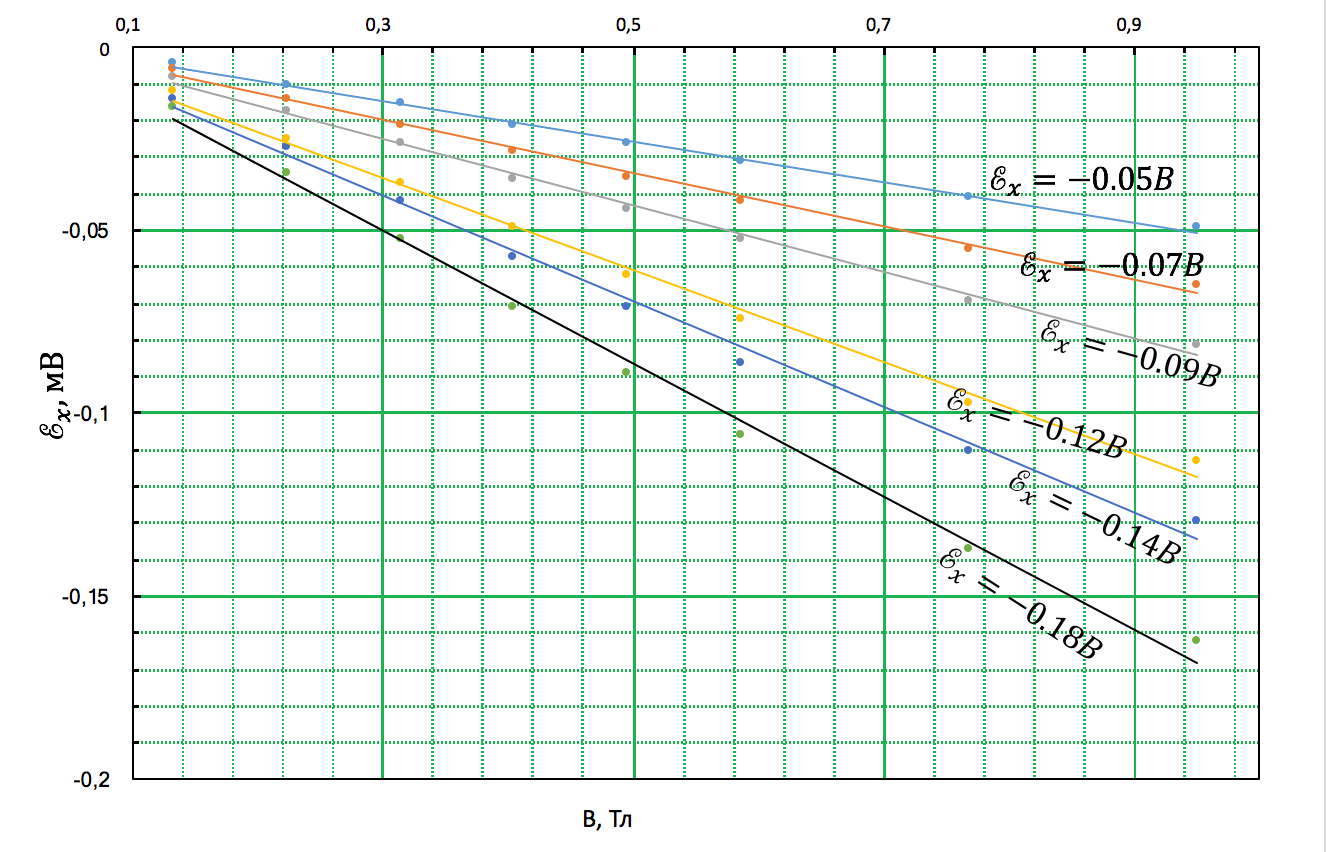
\includegraphics[width = 0.9 \textwidth]{Graph}
			\caption{Построим по полученным данным график зависимости $\mathscr{E}_x = f(B)$ для разных $I$}
		\end{center}
	\end {figure}

$$U_{35} = -1.72 \;\text{мВ}$$

	\begin {figure}[H]
		\begin{center}
		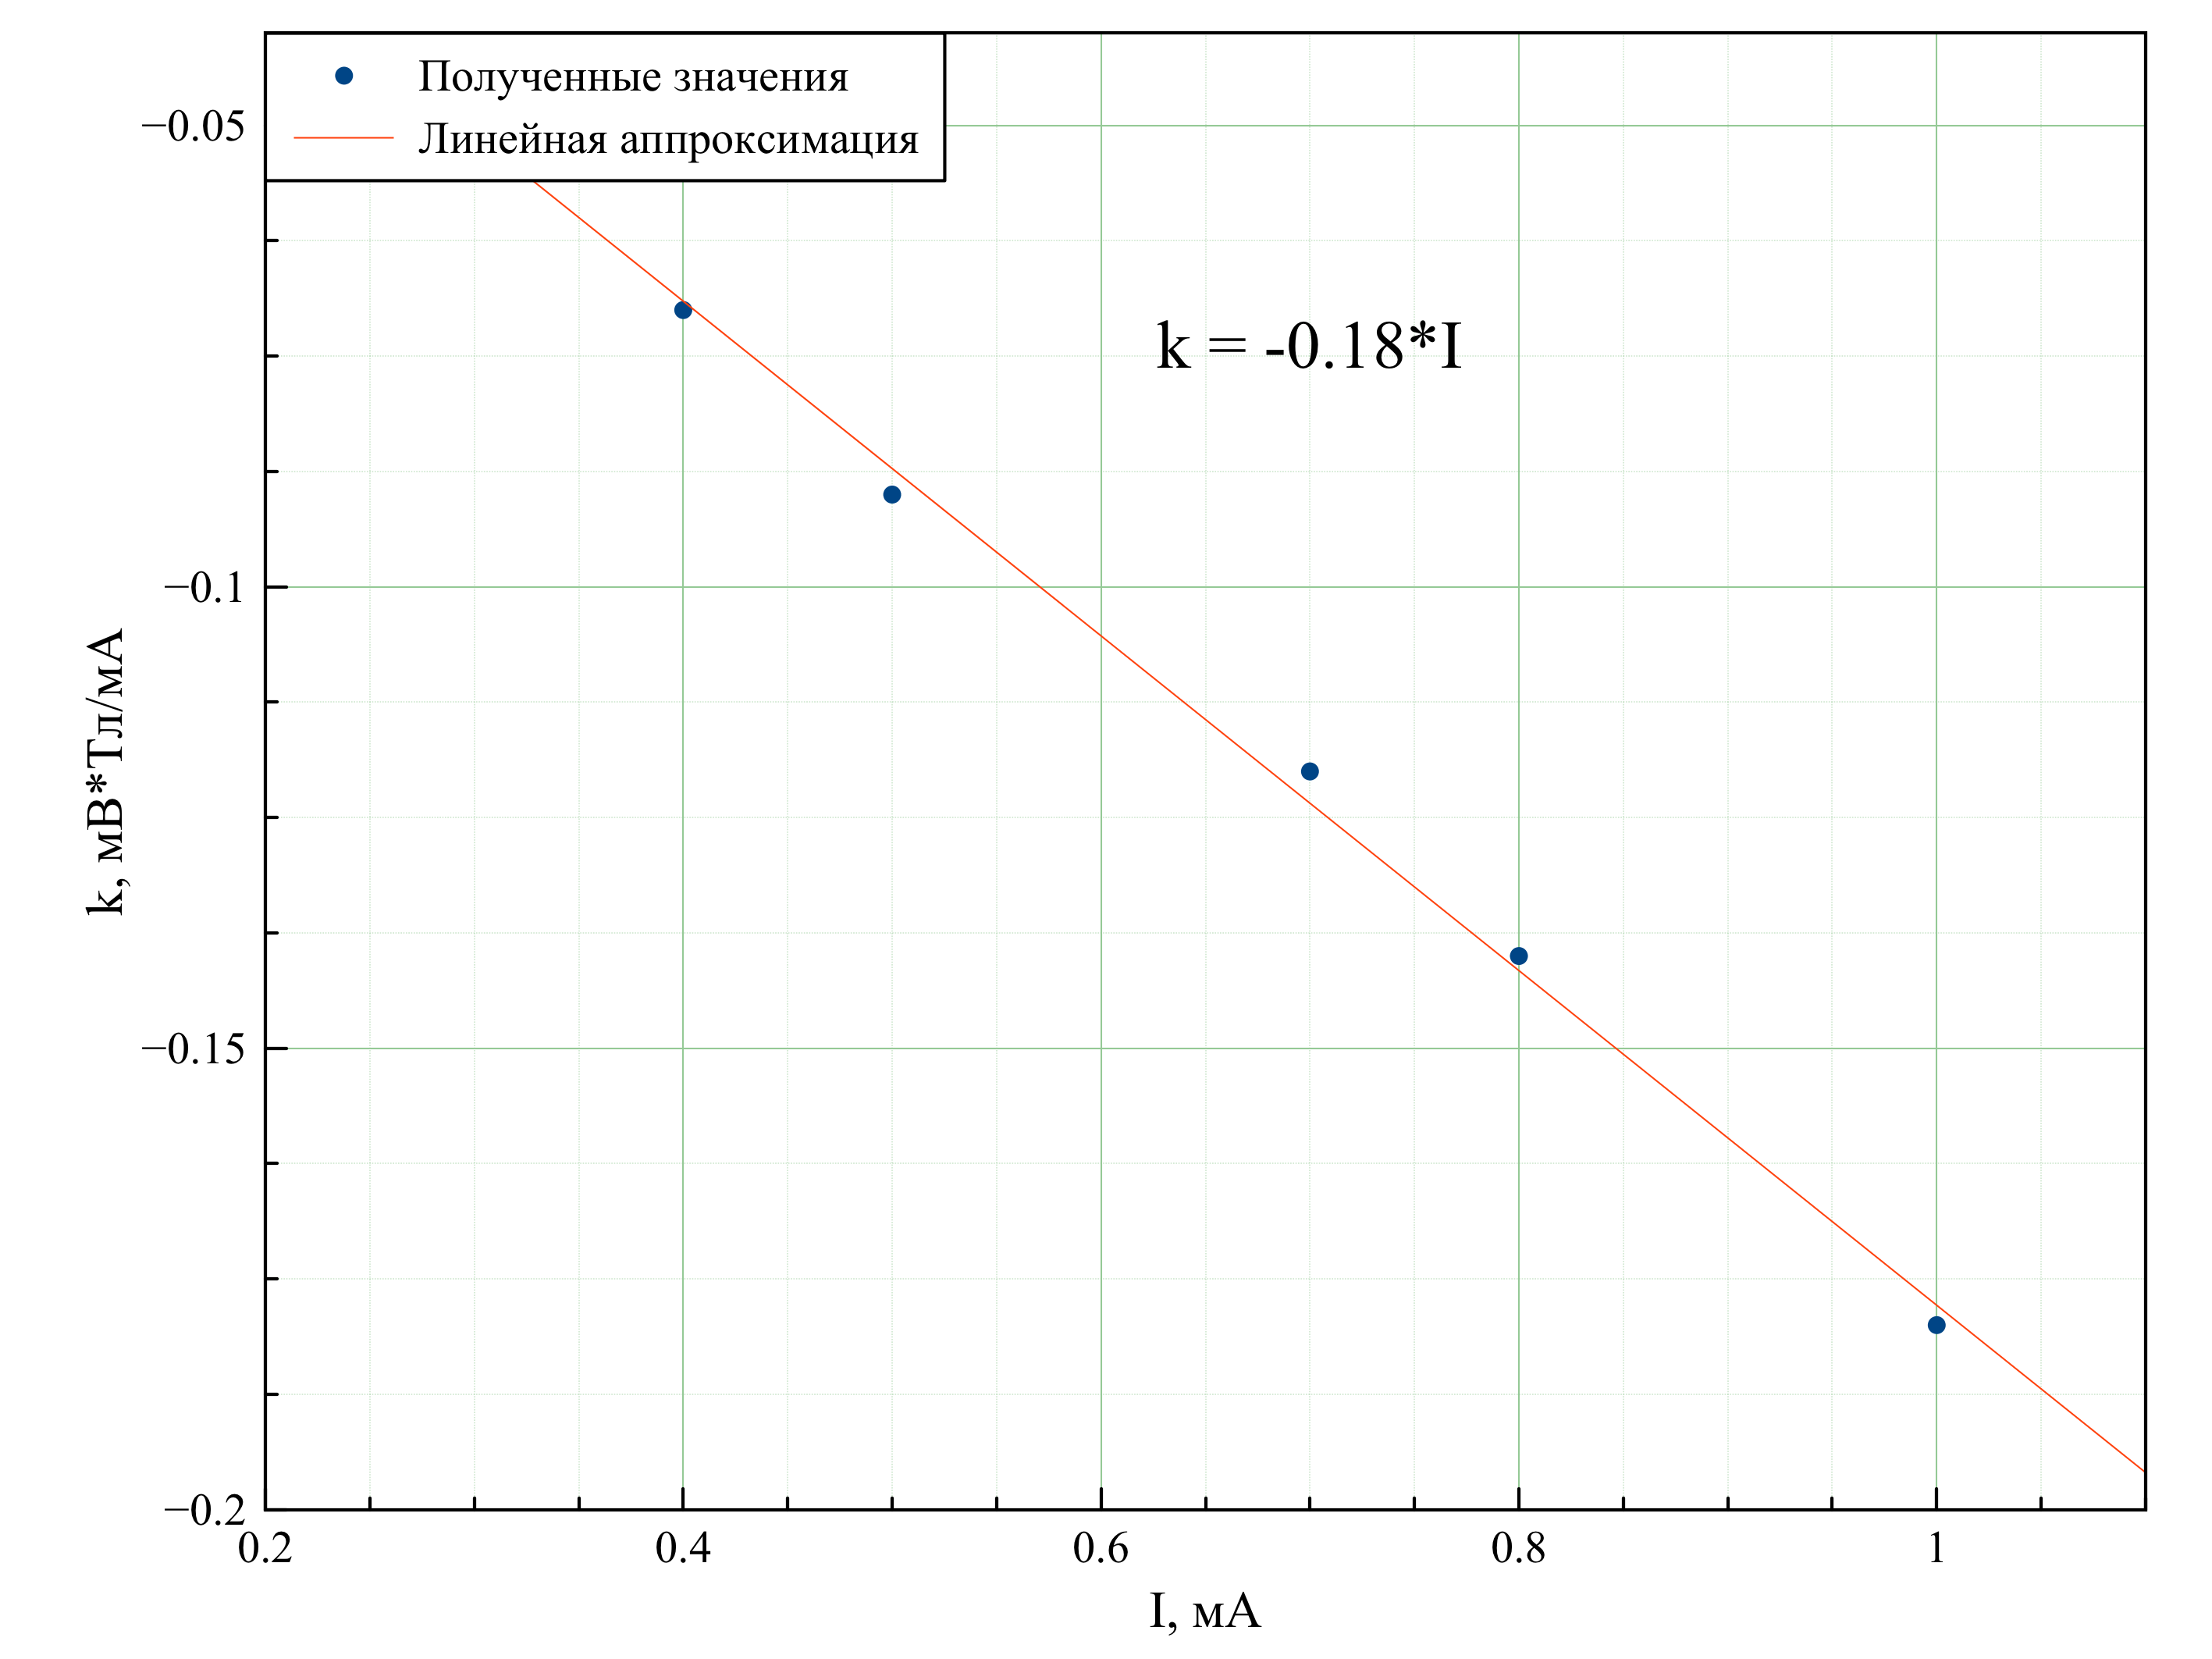
\includegraphics[width = 0.8 \textwidth]{Angle}
			\caption{Построим по полученным углам наклона график зависимости $k = f(I)$}
		\end{center}
	\end {figure}

Тогда  $k_2	 = -(181 \pm 3) \dfrac{\text{мкВ} \cdot \text{Тл}}{\text{мА}}$

Определим постоянную Холла: $R_x = \dfrac{\mathscr{E}_x}{IB} \cdot a = - k_2 \cdot a = (398 \pm 12) \cdot 10^{-6}\; \text{}$

Определим концентрацию носителей заряда: $n = \dfrac{1}{eR_x} = (1.5 \pm 0.1) \cdot 10^{22} \; 1/\text{м}^3$
	
Вычислим удельную проводимость материала: 

$\sigma = \dfrac{I L_{35}}{U_{35} al} = (0.3 \pm 0.01) \cdot 10^3 $ 1/Ом $\cdot$ м  $\left[ \dfrac{\text{См}}{\text{м}} \right]$

Рассчитаем подвижность электрона:
$b = \dfrac{\sigma}{en} = (1.24 \pm 0.05) \cdot 10^3 \dfrac{\text{см}^2}{\text{В} \cdot \text{с}}$

\section{Вывод}

Мы определили постоянную Холла для Германия. Полученная проводимость n-типа. Измерили подвижность и концентрацию заряда в полупроводниках.

\end{document}
